\begin{center}
  \Large
  \textbf{BIOGRAFI PENULIS}
\end{center}

\addcontentsline{toc}{chapter}{BIOGRAFI PENULIS}

\vspace{2ex}

\begin{wrapfigure}{L}{0.3\textwidth}
  \centering
  \vspace{-3ex}
  % Ubah file gambar berikut dengan file foto dari mahasiswa
  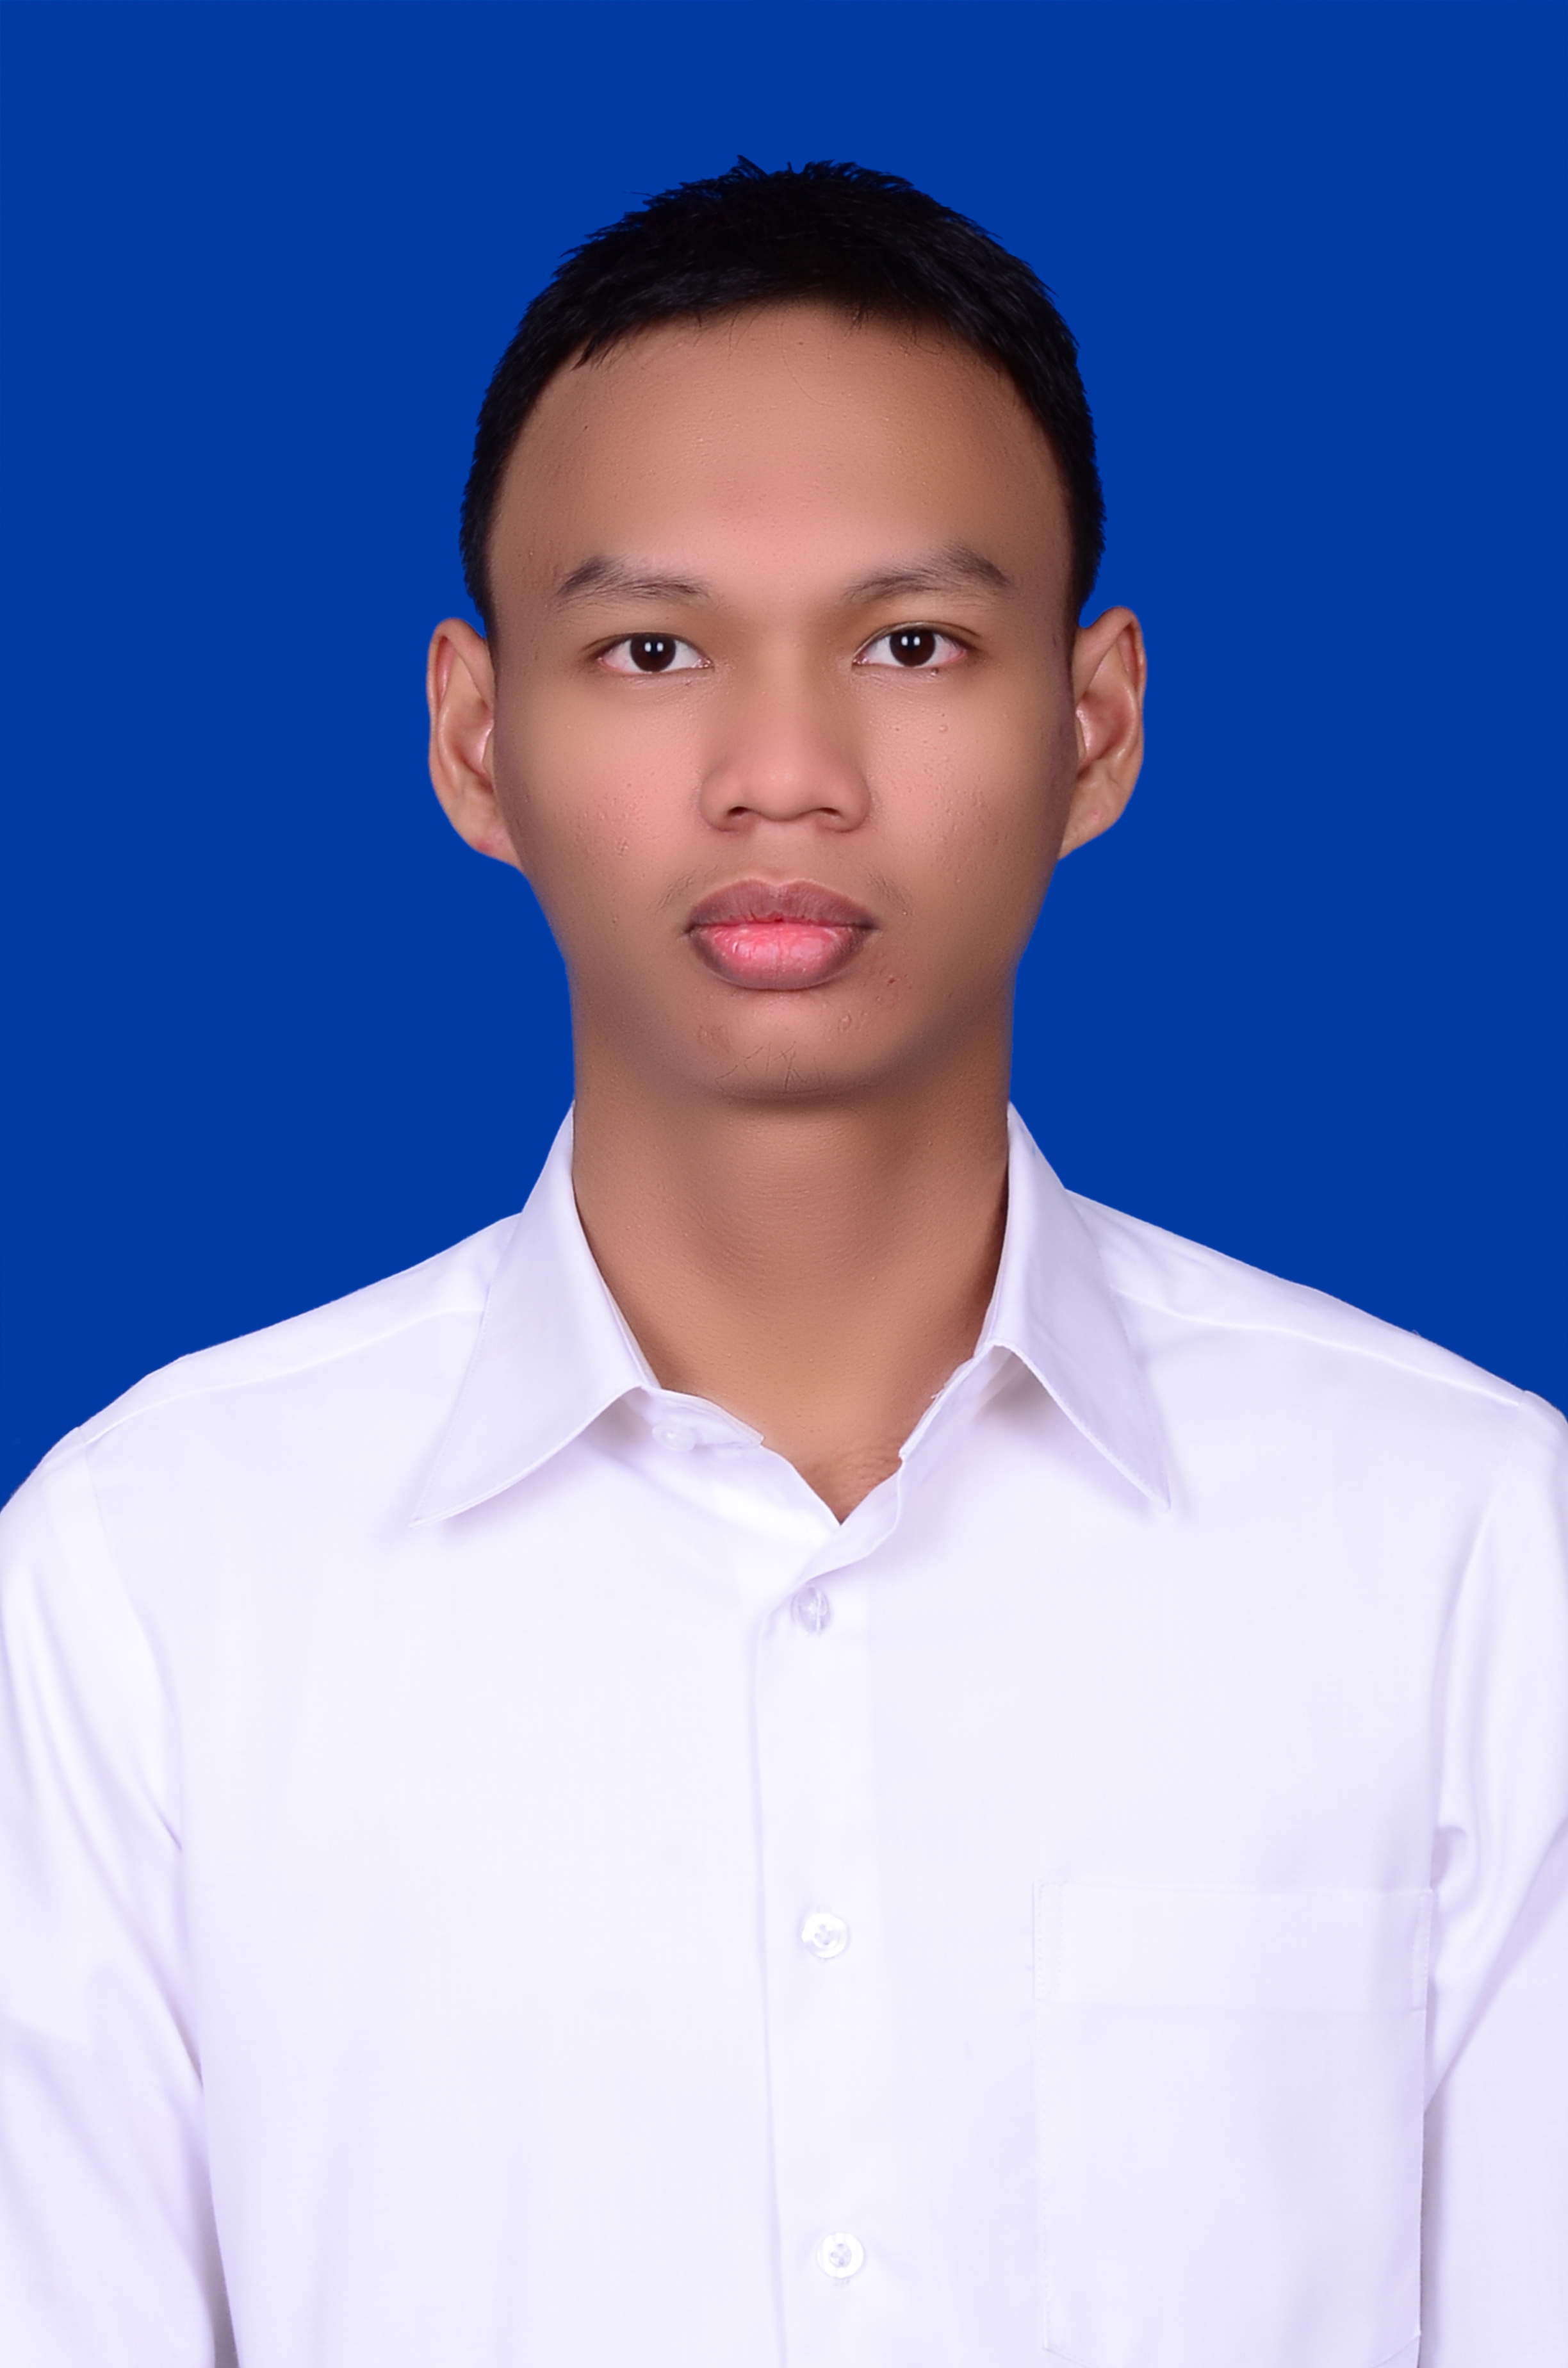
\includegraphics[width=0.3\textwidth]{gambar/Foto Bio.jpg}
  \vspace{-4ex}
\end{wrapfigure}

% Ubah kalimat berikut dengan biografi dari mahasiswa
\name{}, lahir pada tanggal 14 Mei 2001 di Kota Semarang, Jawa Tengah. Merupakan anak kedua dari 
dua bersaudara. Setelah lulus dari SMAN 1 Semarang, penulis melanjutkan pendidikan ke jenjang 
Perguruan Tinggi di program Strata 1 (S1) Departemen Teknik Komputer, Fakultas Teknologi Elektro 
dan Informatika Cerdas (FTEIC), Institut Teknologi Sepuluh Nopember (ITS) Surabaya. Selama berkuliah, 
penulis mengikuti berbagai kegiatan akademis seperti menjadi asisten laboratorium B401, asisten 
praktikum Rangkaian Digital 2022, menjadi peserta Bangkit pada program Bangkit Academy 2022 dengan path 
Pembelajaran Android, dan mencoba program magang kampus merdeka sebagai Quality Assurance di perusahaan 
XL Axiata Tbk. Selain kegiatan akademis, penulis juga mengikuti kegiatan non-akademis seperti menjadi 
staf di UKM IMA (ITS Muay Thai Association), Multimedia and Game Event 6 (MAGE 6), MAGE 7, dan menjadi 
staf pada departemen Hubungan Luar HIMATEKKOM ITS. Selama berkuliah, penulis selalu mencoba untuk menyapa, 
tersenyum, dan berkomunikasi dengan orang-orang sekitar, serta berpikir positif terhadap segala yang terjadi. 
Dalam masa perkuliahan, penulis tertarik mencoba berbagai macam bidang seperti pengembangan aplikasi android, 
games, Internet of Things, dan machine learning, dan pada penelitian Tugas Akhir, penulis memilih untuk 
mencoba penelitian dibidang machine learning.
